\documentclass[10pt,a4paper]{article}
\usepackage[utf8]{inputenc}
\usepackage{amsmath}
\usepackage{amsfonts}
\usepackage{amssymb}
\usepackage{graphicx}
\usepackage[left=2cm,right=2cm,top=2cm,bottom=2cm]{geometry}
\author{Huy Bui}
\title{Internet of Things}
\begin{document}

\section{Introduction}

\subsection{Building Blocks of an IoT System}

A \textbf{sensor} is a device that can be used to measure a physical property by detecting some type of information from the physical world. A sensor may be connected to a controller either directly or remotely.\\

An \textbf{actuator} is a basic motor that can be used to control a system. It can be responsible for transforming an electrical signal into physical output.\\

Controllers are responsible for collecting data from sensors and providing network connectivity. It may have the ability to make immediate decisions (fog computing).\\

A simple IoT system include sensors connecting, through a wireless or wired connection, to actuators or controllers.

\subsection{Processes in Controlled Systems}

Control Systems includes a controller that uses inputs and outputs to manage and regulate the behavior of the system in an attempt to achieve a desired state. The controlled portion of the system is often called the plant.\\

\textbf{Open-loop} control systems do not use feedback. The plant performs a predetermined action without any verification of the desired results. Open-loop control systems are often used for simple processes.\\

\textbf{Feedback loops} are used to provide real-time information to its controller based on current behavior. \\

In a \textbf{closed loop}, feedback is continuously being received by the controller from its sensors. The controller continuously analyzes and processes information, and use actuators to modify conditions.\\

\subsection{Models of Communication}

Both OSI and TCP/IP models are used to describe network connections and often used interchangeably. A similar framework was developed for IoT deployments, that is IoT World Forum Reference Model (Figure \ref{IoT-World-Forum-Reference-Model})


\begin{figure}[hbtp]
\caption{IoT World Forum Reference Model}\label{IoT-World-Forum-Reference-Model}
\centering
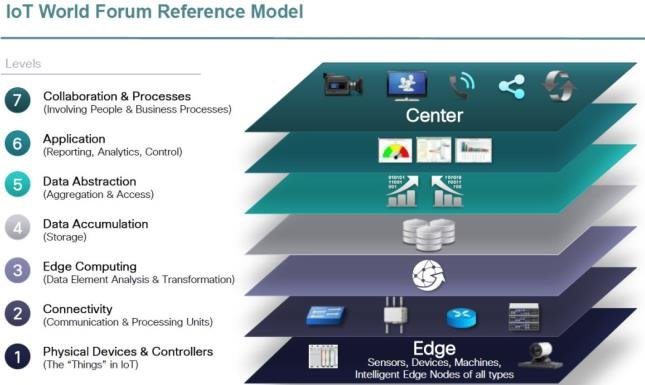
\includegraphics[scale=1]{IoT-World-Forum-Reference-Model.png}
\end{figure}


\end{document}